%!TEX root = ../main.tex

\documentclass[../main.tex]{subfiles}
\begin{document}

\chapter{Conclusions and Future Work}
\label{chapter:future_work}

In this thesis, we study two coverage problems. The first problem is a single agent coverage path planning problem with minimum turns. The objective of this problem is to compute a path that covers the entire workspace and has the minimum number of turns. A greedy algorithm is proposed that achieves a local minimal solution via an iterative re-optimizing decomposition. 

The second part of the thesis tackles a multi-agent coverage path planning problem. The objective of the problem is to plan a coverage path for a team of robots such that the entire workspace is covered and the maximum coverage cost between all robots in the team is minimized. An approximation for the cost of the path is developed and an efficient algorithm is proposed. This approximation is used to partition the workspace into a set of regions assigned to each robot individually. The remainder of the problem solves a single agent coverage problem for each robot individually.

\section{Future Work on Single Agent Coverage}
\label{section:future_single}

There are several potential modifications that would reduce the computational load of the algorithm. The most computational intensive task in Algorithm~\ref{alg:optimal_cut} is computing the cut candidates for each pair of altitude directions (Line~\ref{line:opt_cut_for}-\ref{line:opt_cut_end_for}). The computation load can be reduced by only evaluating a subset of direction pairs as follows.

Define $\underline{W}_{\ell}$ and $\underline{W}_{r}$ to be the polygons on either side of the cone of bisection. It is important to note that the cone of bisection is not a part of these polygons. We compute look-up tables of altitudes for every direction for $\underline{W}_{\ell}$ and $\underline{W}_{r}$ separately such that $\alpha(\underline{W}_{\ell},\text{dir}_1)$ returns the altitude of $\underline{W}_{\ell}$ in direction $\text{dir}_1$. These look-up tables represent the best case scenario for a pair of directions. In the main loop of Algorithm~\ref{alg:optimal_cut}, we keep track of the best altitude so far. A check is added to the main loop such that for a pair of directions, $\text{dir}_1$ and $\text{dir}_2$, if $\alpha(\underline{W}_{\ell},\operatorname{dir}_1)+\alpha(\underline{W}_{r},\operatorname{dir}_2)$ is larger than the best altitude so far, then this pair of directions cannot be optimal, and no further computation is needed.

Also, the quality of the path produced by the proposed method can be increased via an improved sampling. The paths generated by the proposed method may exhibit some undesirable properties  that complicate the transitions between cells. An example of such paths is shown in Figure~\ref{fig:cell_transition}, where the thick dashed line represents a transition that is very costly. A better alternative is to resample the long line closest to the adjacent cell to allow for more \emph{elegant} transitions. An example if shown in Figure~\ref{fig:cell_transition_better}. This method avoids long and costly transitions between cells.

\begin{figure}
	\centering
	\subfile{img/chapter_6/cell_transitions}
	\caption{An example of a undesired cell transition.}
	\label{fig:cell_transition}
\end{figure}

\begin{figure}
	\centering
	\subfile{img/chapter_6/cell_transitions_better}
	\caption{An example of a improvement to inter-cell transitions.}
	\label{fig:cell_transition_better}
\end{figure}


\section{Improvements to Multi-Agent Coverage}
\label{section:future_multi}

One of the main mechanisms for re-optimization is the search for an improving pair-wise cut for two polygons. In this work, the search is limited to a cone of bisection for all reflex vertices. There is no guarantee that the search space of this approach contains the optimal. Considering other search techniques could prove to be beneficial in aiding the search for optimal cuts. For example, by also considering cuts outside the cone of bisection, the search space is increased and the chances of finding an optimal cut are improved. Also, better search techniques could be used to improve the computational burden of the algorithm, i.e., binary search. Better techniques could results in few iterations requires to converge to a minimum, thus reducing the computational burden.

The main limitation of Algorithm~\ref{alg:optimization_procedure} is the greedy nature of choosing neighbors to the current cell for re-optimization. That is, a neighboring cell is chosen only if it has a lower cost compared to the current cell. This condition creates a possibility of a situation where the proposed algorithm terminates but there are modifications to the decompositions that are still possible. An example is provided in Figure~\ref{figure:algo_stuck} where the nodes represent cells, the edges represent adjacency between cells, and the number represent the value of metric $\chi$. Suppose that no cut exists for cells with costs of ten and three. The proposed algorithm will terminate after one iteration. However, it is possible that by making a cut for cells with cost three and seven such that the cost of seven is increases slightly, the changes in the decomposition allows for a new cut between ten and three that reduces the global maximum cost.

\begin{figure}
	\centering
	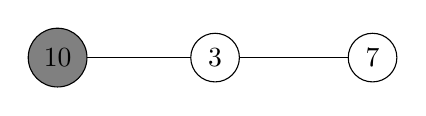
\begin{tikzpicture}
		\draw [->] (0,5)--(2,5);
		\draw [->] (2,5)--(4,5);

		\node[draw, circle, fill=gray] at (0,5) {$10$};
		\node[draw, circle, fill=white] at (2,5) {$3$};
		\node[draw, circle, fill=white] at (4,5) {$7$};

	\end{tikzpicture}
	\caption{An example where the current re-optimization technique terminates.}
	\label{figure:algo_stuck}
\end{figure}

  %In this thesis, a recursive algorithm was proposed that searches for improving cuts between the highest cost cell and its neighbors. If such a cut is not found, the algorithm searches for a cut for the neighbors for the purpose of modifying the neighbors enough to allow for improvement in the highest cost cell. However, there are other approaches to achieve this goal.


\end{document}